
\begin{enumerate}
    \item A train S1, moving with a uniform velocity of 108 km/h, approaches another train S2 standing on a platform. An observer O moves with a uniform velocity of 36 km/h towards S2, as shown in figure. Both the trains are blowing whistles of same frequency 120 Hz. When O is 600 m away from S2 and distance between S1 and S2 is 800 m, the number of beats heard by O is \_\_\_\_\_\_\_\_\_. \\
    [Speed of the sound = 330 m/s]
    \begin{center}
        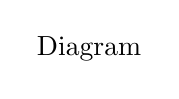
\begin{tikzpicture}
            \node {Diagram};
        \end{tikzpicture}
    \end{center}
\end{enumerate}
